\documentclass[11pt]{article}

\usepackage[margin=1in]{geometry}
\usepackage{amsmath, amssymb}
\usepackage{booktabs}
\usepackage{graphicx}
\usepackage{listings}

\title{EE/CS 148B HW2}
\author{Yash Kakade}
\date{\today}

\begin{document}

\maketitle

\section{Problem 2.3 -- Simple Profiling}

\subsection*{Part 1}

The benchmarking script is \texttt{systems/benchmark.py}.
The core measurement loop (simplified) is:

\begin{lstlisting}[language=Python]
# warmup
for _ in range(config.warmup_steps):
    run_single_step(model, batch, config.mode, autocast_ctx, optimizer)

# measure
step_times = []
for _ in range(config.measure_steps):
    start = timeit.default_timer()
    run_single_step(model, batch, config.mode, autocast_ctx, optimizer)
    step_times.append(timeit.default_timer() - start)
# run_single_step calls torch.cuda.synchronize() before returning
\end{lstlisting}

\subsection*{Part 2}

\begin{table}[h]
\centering
\begin{tabular}{lcc}
\toprule
Model & Forward Time & Backward Time \\
\midrule
Small & $0.3421 \pm 0.0345$ s & $1.7290 \pm 0.0244$ s \\
Medium & $1.3798 \pm 0.5713$ s & $2.0685 \pm 0.0454$ s \\
Large & $2.9783 \pm 0.0599$ s & $7.0291 \pm 0.1196$ s \\
\bottomrule
\end{tabular}
\end{table}

Backward passes are 5--8$\times$ slower than forward across all model sizes, since backprop traverses the full computation graph plus gradient accumulation. Variance was low except for the medium forward pass.

\subsection*{Part 3}

\begin{table}[h]
\centering
\begin{tabular}{llcc}
\toprule
Warmup Steps & Model & Forward Time & Backward Time \\
\midrule
0 & Small & $0.3919 \pm 0.1448$ s & $0.7164 \pm 0.0262$ s \\
0 & Medium & $0.9452 \pm 0.1299$ s & $2.0262 \pm 0.0413$ s \\
0 & Large & $3.0873 \pm 0.1504$ s & $6.8241 \pm 0.0947$ s \\
1 & Small & $0.8019 \pm 0.0149$ s & $1.6784 \pm 0.0327$ s \\
1 & Medium & $1.2190 \pm 0.1980$ s & $4.6955 \pm 0.3864$ s \\
1 & Large & $7.3462 \pm 0.2021$ s & $15.8415 \pm 0.7451$ s \\
2 & Small & $0.7809 \pm 0.0327$ s & $1.6364 \pm 0.0954$ s \\
2 & Medium & $2.1242 \pm 0.0188$ s & $2.4386 \pm 0.7010$ s \\
2 & Large & $3.2859 \pm 0.1609$ s & $8.7790 \pm 3.3968$ s \\
10 & Small & $0.3430 \pm 0.0200$ s & $0.7427 \pm 0.0281$ s \\
10 & Medium & $1.4703 \pm 0.5285$ s & $2.3188 \pm 0.0888$ s \\
10 & Large & $3.2096 \pm 0.1037$ s & $4.8267 \pm 0.0693$ s \\
\bottomrule
\end{tabular}
\end{table}

The large backward without warmup jumped from 6.8 s (0 steps) to 15.8 s (1 step) before settling at 4.8 s with 10 steps---a 3$\times$ swing. The instability is from CUDA lazy initialization and kernel autotuning on the first few calls. With 1--2 warmup steps things were still inconsistent; 10 steps mostly converged, though some forward timings still varied.

%%%%%%%%%%%%%%%%%%%%%%%%%%%%%%%%%%%%%%%%%%%%%%%%%%

\section{Problem 2.4 -- Nsight Profiling}

\subsection*{Part 1}

For the small model (ctx=128), the forward-pass NVTX range was 26.3 ms in Nsight, lower than the Python timer average because this captured a single steady-state step. The dominant kernel was \texttt{ampere\_sgemm\_128x64\_tn} (cuBLAS GEMM), totaling 81.8 ms cumulatively over 6 forward passes ($\approx$57 calls each). The remaining GPU time went to softmax reductions, elementwise ops, and attention masking.

Adding backward, the same GEMM kernel stayed on top (76 ms), joined by \texttt{ampere\_sgemm\_128x64\_nn} (63 ms) and \texttt{\_nt} (58 ms) for the weight/activation gradients, plus more elementwise work.

A full AdamW training step measured 134.6 ms total: 44.9 ms forward, 50.3 ms backward, 46.6 ms optimizer. The optimizer step is nearly as expensive as forward because AdamW applies a fused elementwise update to every parameter---GEMM fraction drops compared to inference.

Inside self-attention, softmax (22.6 ms) took more time than the score matmul (12.6 ms) or output matmul (5.9 ms) despite far fewer FLOPs. Softmax is memory-bandwidth limited and involves several small kernels (max, exp, sum, divide), which cuBLAS GEMMs don't have.

% insert profiler screenshot here

%%%%%%%%%%%%%%%%%%%%%%%%%%%%%%%%%%%%%%%%%%%%%%%%%%

\section{Problem 2.5 -- Mixed Precision}

\subsection*{Accumulation Experiment}

Adding 0.01 a thousand times: FP32+FP32 gives \texttt{10.0001} (accurate), FP16+FP16 gives \texttt{9.9531} (off by 0.05), and FP32 accumulator with FP16 addends gives \texttt{10.0021} (with or without explicit cast). Pure FP16 loses precision because once the sum is $\sim\!1$, the FP16 grid is too coarse to represent 0.01 exactly and additions get rounded away. Keeping the accumulator in FP32 mostly fixes this---FP32's mantissa is wide enough to add 0.01 to 10 without losing it.

\subsection*{Part 1 -- Datatypes under FP16 Autocast}

\begin{table}[h]
\centering
\begin{tabular}{lc}
\toprule
Component & Datatype \\
\midrule
Model parameters (within autocast context) & \texttt{float32} \\
Output of \texttt{fc1} (first linear + ReLU) & \texttt{float16} \\
Output of \texttt{ln} (layer norm) & \texttt{float32} \\
Model logits (\texttt{fc2} output) & \texttt{float16} \\
Loss & \texttt{float32} \\
Gradients & \texttt{float32} \\
\bottomrule
\end{tabular}
\end{table}

\subsection*{Part 2 -- Layer Norm and BF16}

Under FP16 autocast, layer norm runs in FP32 because summing squared activations for variance can overflow FP16's $\pm 65504$ range. BF16 removes that overflow risk (same dynamic range as FP32), but PyTorch still runs layer norm in FP32 under BF16 autocast---BF16's 7-bit mantissa is actually shorter than FP16's 10 bits, so rounding error in the variance estimate is worse, not better.

\subsection*{Part 3 -- BF16 Benchmarking Results}

\begin{table}[h]
\centering
\begin{tabular}{lcccccc}
\toprule
Model & FP32 Fwd (s) & BF16 Fwd (s) & Speedup & FP32 Bwd (s) & BF16 Bwd (s) & Speedup \\
\midrule
Small  & $0.342 \pm 0.035$ & $0.143 \pm 0.008$ & $2.4\times$ & $1.729 \pm 0.024$ & $0.201 \pm 0.023$ & $8.6\times$ \\
Medium & $1.380 \pm 0.571$ & $0.291 \pm 0.015$ & $4.7\times$ & $2.069 \pm 0.045$ & $0.314 \pm 0.021$ & $6.6\times$ \\
Large  & $2.978 \pm 0.060$ & $0.584 \pm 0.044$ & $5.1\times$ & $7.029 \pm 0.120$ & $0.486 \pm 0.068$ & $14.5\times$ \\
\bottomrule
\end{tabular}
\caption{FP32 vs.\ BF16 autocast timing (5 warmup, 10 measured steps, ctx=128, batch=4).}
\end{table}

BF16 is 2--5$\times$ faster on forward and 7--15$\times$ on backward, with larger gains at larger model sizes. Bigger models spend more of their time in large GEMMs, which Tensor Cores hit hardest. Backward gets an even bigger jump because it has more GEMMs per layer (gradients for both weights and activations) and benefits from reduced memory traffic as well.

%%%%%%%%%%%%%%%%%%%%%%%%%%%%%%%%%%%%%%%%%%%%%%%%%%

\section{Problem 2.6 -- Memory Profiling}

\subsection*{Part 1}

\begin{figure}[h]
\centering
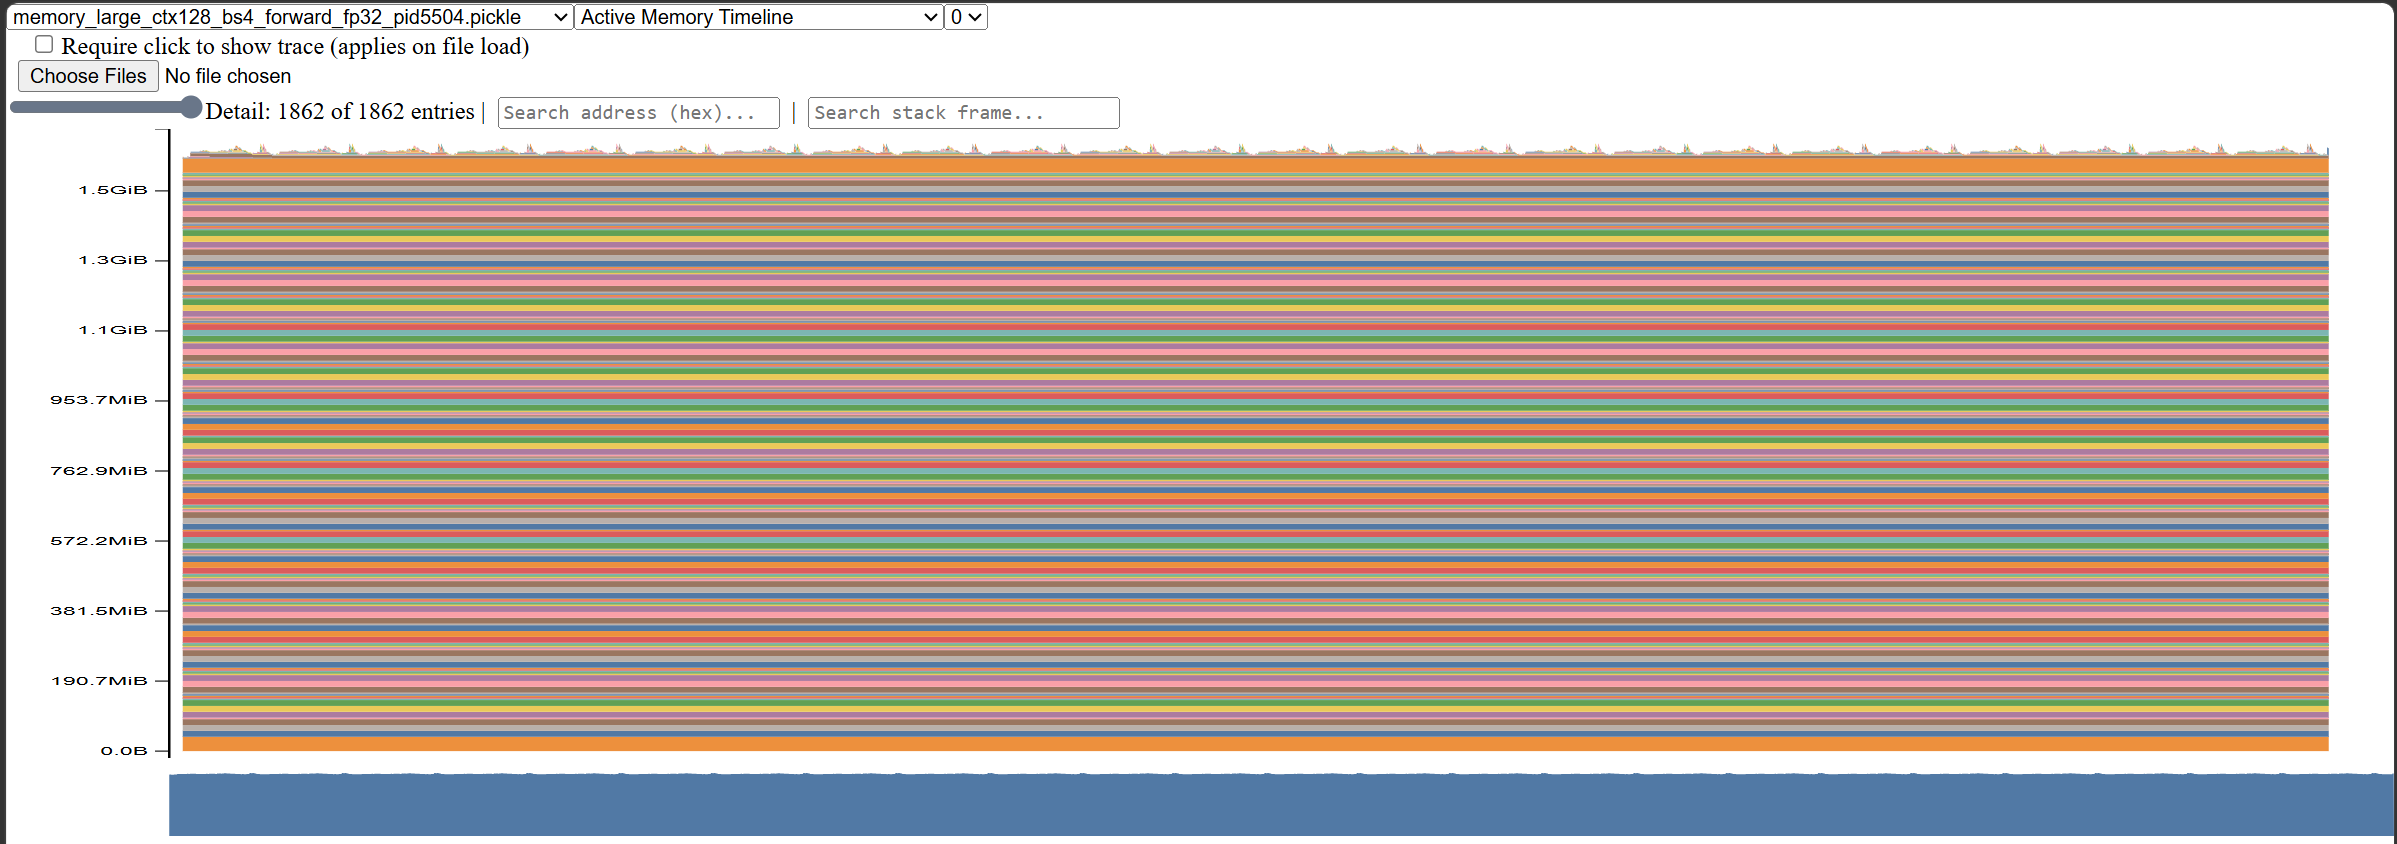
\includegraphics[width=\textwidth]{artifacts/memory/memory_large_ctx128_bs4_forward_fp32_pid5504.png}
\caption{Active memory timeline for a forward-only pass of the large model at context length 128.}
\end{figure}

\begin{figure}[h]
\centering
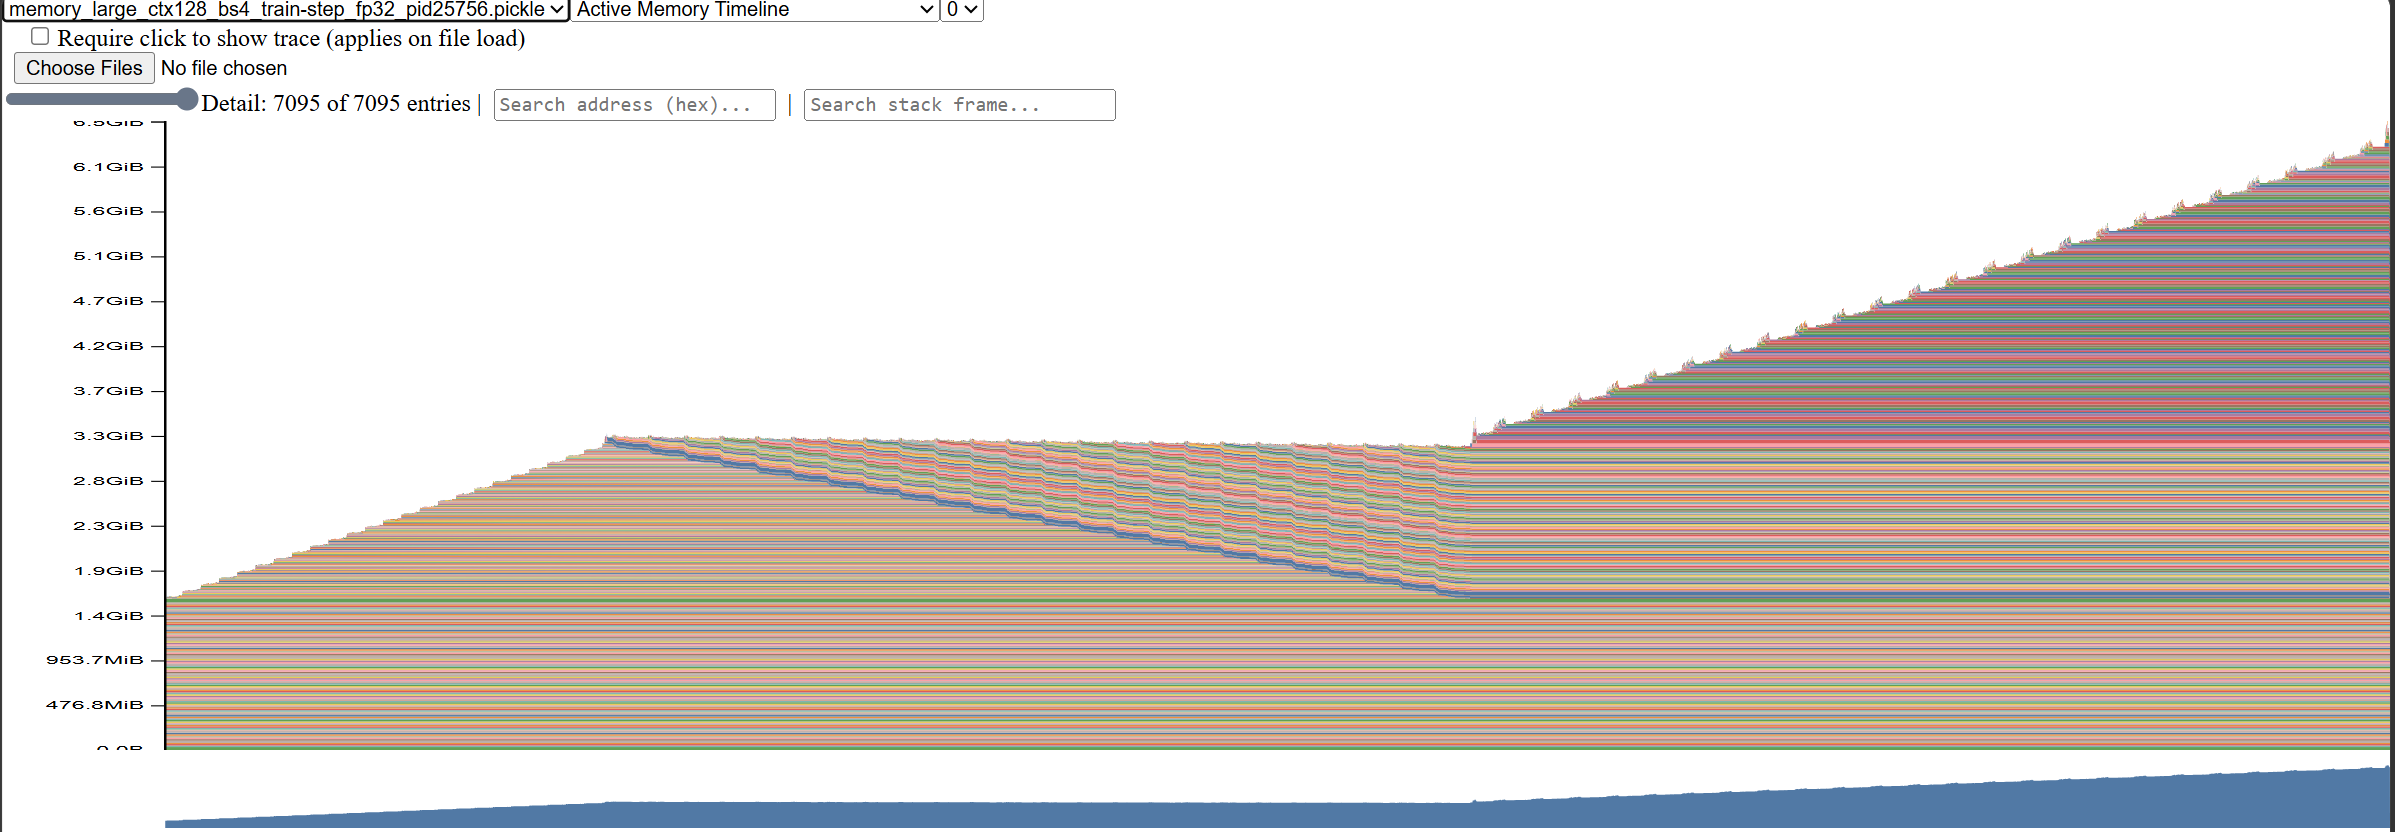
\includegraphics[width=\textwidth]{artifacts/memory/memory_large_ctx128_bs4_train-step_fp32_pid25756.png}
\caption{Active memory timeline for a full training step of the large model at context length 128.}
\end{figure}

The \texttt{--use-memory-profiler} flag starts \texttt{torch.cuda.memory.\_record\_memory\_history} after warmup, profiles one step, and dumps a snapshot to \texttt{artifacts/memory/}. The forward-only timeline is nearly flat---parameters are the baseline and activations are a small bump. The training step is more interesting: memory climbs during forward (saving activations), drops as they're freed during backward, then spikes again when AdamW materializes gradients and optimizer state, peaking around 6.5 GiB.

\subsection*{Part 2}

\begin{table}[h]
\centering
\begin{tabular}{ccc}
\toprule
Context Length & Forward Peak Memory & Training-Step Peak Memory \\
\midrule
128 & 1656.4 MiB & 6701.1 MiB \\
256 & 1708.5 MiB & 6721.1 MiB \\
512 & 1920.8 MiB & 10814.3 MiB \\
1024 & 2729.9 MiB & OOM \\
\bottomrule
\end{tabular}
\end{table}

Forward memory grows slowly because parameters dominate---longer sequences just add a bit more activation memory. Training-step peak is much higher since it also holds saved activations, gradients, and Adam state. At context 1024 the training step OOM'd, likely when attention scores across all layers couldn't fit alongside gradients.

\subsection*{Part 3}

BF16 didn't meaningfully reduce peak memory. The training-step peak was essentially the same (6690 vs.\ 6701 MiB), and forward actually used \emph{more} (2425 vs.\ 1656 MiB), likely from autocast's cached type conversions. Parameters, gradients, and Adam state all stay in FP32, so the dominant costs don't shrink.

\subsection*{Part 4}

For the large model at the reference hyperparameters, a residual-stream activation
tensor has shape $4 \times 128 \times 1024$. In single precision this is
$4 \cdot 128 \cdot 1024 \cdot 4 = 2{,}097{,}152$ bytes, or exactly $2.0$ MiB
after dividing by $1024^2$.

%%%%%%%%%%%%%%%%%%%%%%%%%%%%%%%%%%%%%%%%%%%%%%%%%%

\section{Problem 2.7 -- Attention Profiling}

\begin{table}[h]
\centering
\small
\begin{tabular}{rrrrr}
\toprule
$d_k$ & Seq Len & Fwd (ms) & Bwd (ms) & Mem before bwd (MB) \\
\midrule
16  &   64 & 1.39 & 4.93 &  8.5 \\
16  &  128 & 1.72 & 4.76 & 17.5 \\
16  &  256 & 1.81 & 4.75 & 20.8 \\
16  &  512 & 1.89 & 4.99 & 33.3 \\
16  & 1024 & 3.60 & 9.03 & 82.3 \\
\midrule
32  &   64 & 1.91 & 4.75 & 16.8 \\
32  &  128 & 1.36 & 5.03 & 17.8 \\
32  &  256 & 1.50 & 4.79 & 21.3 \\
32  &  512 & 2.31 & 5.01 & 34.3 \\
32  & 1024 & 3.96 & 9.36 & 84.3 \\
\midrule
64  &   64 & 1.65 & 5.20 & 17.0 \\
64  &  128 & 1.75 & 4.85 & 18.3 \\
64  &  256 & 1.57 & 4.70 & 22.3 \\
64  &  512 & 2.31 & 5.73 & 36.3 \\
64  & 1024 & 6.75 & 12.98 & 88.3 \\
\midrule
128 &   64 & 1.58 & 5.45 & 17.5 \\
128 &  128 & 1.70 & 3.25 & 19.3 \\
128 &  256 & 0.79 & 2.24 & 24.3 \\
128 &  512 & 2.15 & 4.97 & 40.3 \\
128 & 1024 & 4.69 & 9.57 & 96.3 \\
\bottomrule
\end{tabular}
\caption{Attention profiling: batch size 8, single head. All configurations ran without OOM on the RTX 3050 Ti (4 GB).}
\end{table}

Nothing OOM'd on this machine---standalone attention is much leaner than the full model, with the largest config ($d_k=128$, seq=1024) using only 96 MB before backward. Memory scales quadratically: the attention score matrix is $(\text{batch} \times \text{heads} \times s^2 \times 4)$ bytes, so it goes from 1 MB at $s=64$ to 256 MB at $s=1024$. On a 24 GB GPU with a full model, this is what kills long contexts.

Runtime follows the same trend: forward time roughly doubles from $s=512$ to $s=1024$ for $d_k \ge 64$ (consistent with 4$\times$ FLOPs). At short lengths, kernel launch overhead dominates and timings are mostly flat.

Flash Attention eliminates the quadratic memory cost by computing $QK^\top$ in SRAM tiles, so the full $s \times s$ score matrix is never written to HBM. Backward memory drops from $O(s^2)$ to $O(s)$ at the cost of recomputing scores on the backward pass.

%%%%%%%%%%%%%%%%%%%%%%%%%%%%%%%%%%%%%%%%%%%%%%%%%%

\section{Problem 2.8 -- Torch Compile}

\subsection*{Part 1 -- Compiled Attention}

\textbf{Note on backend:} The default \texttt{inductor} backend for \texttt{torch.compile} requires Triton, which is not available on Windows. All results below use \texttt{backend="aot\_eager"}, which performs AOT autograd tracing but does not fuse CUDA kernels.

\begin{table}[h]
\centering
\small
\begin{tabular}{rrrrrrr}
\toprule
$d_k$ & Seq Len & Fwd (ms) & Bwd (ms) & Compiled Fwd (ms) & Compiled Bwd (ms) & Fwd Slowdown \\
\midrule
16  &   64 &  1.39 &  4.93 &  6.48 & 12.81 & $4.7\times$ \\
16  & 1024 &  3.60 &  9.03 & 26.55 & 59.71 & $7.4\times$ \\
64  &   64 &  1.65 &  5.20 &  7.12 & 12.66 & $4.3\times$ \\
64  & 1024 &  6.75 & 12.98 & 27.27 & 60.79 & $4.0\times$ \\
128 &   64 &  1.58 &  5.45 &  8.96 & 12.84 & $5.7\times$ \\
128 & 1024 &  4.69 &  9.57 & 27.39 & 62.00 & $5.8\times$ \\
\bottomrule
\end{tabular}
\caption{Selected attention configurations: uncompiled (§2.7) vs.\ compiled (\texttt{aot\_eager}), batch=8, heads=1.}
\end{table}

Everything got slower. Without Triton (Linux-only), \texttt{aot\_eager} can't fuse any kernels---it just adds AOT dispatch overhead on top of eager execution. Slowdown is worst at short sequences (5--7$\times$) where the overhead swamps the actual work, and still 4--6$\times$ at seq=1024.

\subsection*{Part 2 -- Compiled Full Transformer}

\begin{table}[h]
\centering
\begin{tabular}{lccccc}
\toprule
Model & Vanilla Fwd (s) & Compiled Fwd (s) & Fwd $\Delta$ & Vanilla Train (s) & Compiled Train (s) & Train $\Delta$ \\
\midrule
Small  & $0.038 \pm 0.007$ & $0.148 \pm 0.034$ & $3.9\times$ slower & $0.681 \pm 0.024$ & $0.365 \pm 0.066$ & $1.9\times$ faster \\
Medium & $0.091 \pm 0.026$ & $0.197 \pm 0.042$ & $2.2\times$ slower & $1.778 \pm 0.023$ & $0.620 \pm 0.076$ & $2.9\times$ faster \\
Large  & $0.220 \pm 0.065$ & $0.663 \pm 0.164$ & $3.0\times$ slower & $15.34 \pm 3.34$ & $23.74 \pm 3.33$ & $1.5\times$ slower \\
\bottomrule
\end{tabular}
\caption{Vanilla vs.\ \texttt{torch.compile} (\texttt{aot\_eager}) on the Transformer model; all FP32, ctx=128, batch=4, 5 warmup + 10 measured steps.}
\end{table}

Forward-only is 2--4$\times$ slower for the same reason as Part 1. The training step is more interesting: small and medium get 1.9$\times$ and 2.9$\times$ faster, probably because \texttt{aot\_eager} cuts Python dispatch overhead that's proportionally large in the backward and optimizer step (many small ops). The large model goes the other way---1.5$\times$ slower---likely because it's already over the 4 GiB VRAM (6.7 GiB allocated, spilling into system RAM), and the compiled graph's memory layout worsens the spill.

%%%%%%%%%%%%%%%%%%%%%%%%%%%%%%%%%%%%%%%%%%%%%%%%%%

\section{Problem 3.1 -- GSM8K Baseline}

\begin{lstlisting}[language=Python]
# code here
\end{lstlisting}

Response here.

%%%%%%%%%%%%%%%%%%%%%%%%%%%%%%%%%%%%%%%%%%%%%%%%%%

\section{Problem 3.2 -- Prompting Baselines}

\subsection*{Chain of Thought}

Response here.

\subsection*{Self Consistency}

Response here.

%%%%%%%%%%%%%%%%%%%%%%%%%%%%%%%%%%%%%%%%%%%%%%%%%%

\section{Problem 3.5 -- GRPO}

\subsection*{Training Results}

% insert training curve here

Response here.

\end{document}
